% Tento soubor nahraďte vlastním souborem s obsahem práce.
%=========================================================================
% Autoři: Michal Bidlo, Bohuslav Křena, Jaroslav Dytrych, Petr Veigend a Adam Herout 2019

% Pro kompilaci po částech (viz projekt.tex), nutno odkomentovat a upravit
%\documentclass[../projekt.tex]{subfiles}
%\begin{document}

\newtheorem{definition}{\textbf{Definice}}

\chapter{Úvod}
\label{ch:uvod}

Umělá inteligence je obor, který nás postupem let všechny obkopuje čím dál tím více.
Dokonce je navždy spjata i s naším českým národem, když Karel Čapek dal zrodu slova robot.

Pokrok umělé inteligence je často měřen aplikací v oblasti her.
Hry jsou vhodným ukazatelem pokroku v oblasti umělé inteligence, protože mají jasná pravidla, výkon je snadno měřitelný a pokrok dokáže vidět i lajk.
Umělá inteligence již dokázala porazit nejlepší hráče v šachu~\cite{DeepBlue}, Dota 2~\cite{Dota2} a Go~\cite{AlphaGo}.

Hra studovaná v této práci je hra Scotland Yard.
Je to hra pro tři až šest hráčů.
V této hře obvykle hraje jeden hráč jako Pan X, který se snaží uniknout policistům, ovládanými ostatními hráči.
Policisté avšak nevědí, kde na herním poli se Pan X nachází.
Musí tedy odhadovat jeho pozici a spolupracovat mezi sebou, aby ho mohli polapit.
Pozice Pana X je odhalena pouze v určitých kolech.
Hra končí, když je Pan X chycen (vyhrávají policisté), nebo když je dosažen maximální počet kol (vyhrává Pan X).
Scotland Yard je ideální hrou ke studování umělé inteligence, protože se jedná o hru s nedokonalou informací a k vítězství policistů je zapotřebí spolupráce a strategie.

Zaměření této práce jsem si vybral jelikož mi vždy byla umělá inteligence blízká a vždy jsem chtěl začít tomuto odvětví více věnovat i po praktické stránce.

Tato práce blíže zkoumá algoritmy posilovaného učení, konkrétně algoritmu PPO (Proximal Policy Optimization) a jejich použití na hry s neurčitostí.
Algoritmus PPO je často používán k řešení problémů se spojitými veličinamy a ve 3D prostoru.
Často se využívá ve hrách.
Dle provedených studií je vhodný k řešení problémů s nedokonalou informací~\cite{Manille} a je vhodný pro hry na schování a hledání~\cite{PPO_Hide_Seek}.
Proto je pro mě zajímavý a zkušenost s tímto algoritmém by se dala využít v mém pracovním životě.

Pro zpracování práce byly využity tyto hlavní knihovny:
\begin{itemize}
  \item \emph{Ray.Rlib} - knihovna s implementací algoritmu PPO, použita k učení agenta
  \item \emph{PyTorch} - podpůrná knihovna Ray.Rlib
  \item \emph{TensorFlow} - podpůrná knihovna Ray.Rlib
  \item \emph{Gym} - knihovna sloužící k vytvoření prostředí
  \item \emph{Pygame} - knihovna pro vytváření uživatelského rozhraní
\end{itemize}


\chapter{Shrnutí dosavadního stavu}
\label{ch:dosavadni_stav}
Tato kapitola není encyklopedickým výčtem celého tématu bakalářské práce.
Jedná se avšak o shrnutí nejdůležitějších relevantních informací a pojmů, duležitých pro tuto práci.

\begin{itemize}
  \item \emph {40-50\,\% rozsahu práce}
  \item \emph{Hodně citovat literaturu}
  \item \emph{Vysvětlit všechno, už ne pro plebíky}
  \item \emph{Je vhodné na začátku této části uvést, co obsahuje a proč a taky že „není encyklopedickým přehledem“}
  \item \emph{Asi tak ze 2 kapitol?}
  \item \emph{Existující řešení (implementace scotlandu, říct že se implementuje pomocí tamtoho algoritmu a proč jsem vzal PPO)}
\end{itemize}


\section{Desková hra Scotland Yard}
\label{sec:deskova-hra-scotland-yard}

Scotland Yard je populární hra pro tři a více hráčů, která kombinuje prvky schovávané a hry na honěnou.
Jeden hráč hraje za Pana X, který se snaží uniknout policistům, ovládanými ostatními hráči.
Hra končí, když je Pan X chycen (vyhrávají policisté), nebo když je dosažen maximální počet kol (vyhrává Pan X).
Originální hra se odehrává v Londýně.
Na herní mapě se nachází 200 polí, které jsou vzájemně propojené náhodnými cestami.
Každá cesta povoluje určitý způsob pohybu (např.
pouze taxíkem, pouze autobusem, atd.).
Jednotliví hráči využívají prvky veřejné dopravy k pohybu po herní ploše, kterými jsou:
\begin{itemize}
  \item \emph{Taxi}
  \item \emph{Autobus}
  \item \emph{Metro}
  \item \emph{Trajekt}
\end{itemize}

\begin{figure}[!h]
	\centering
	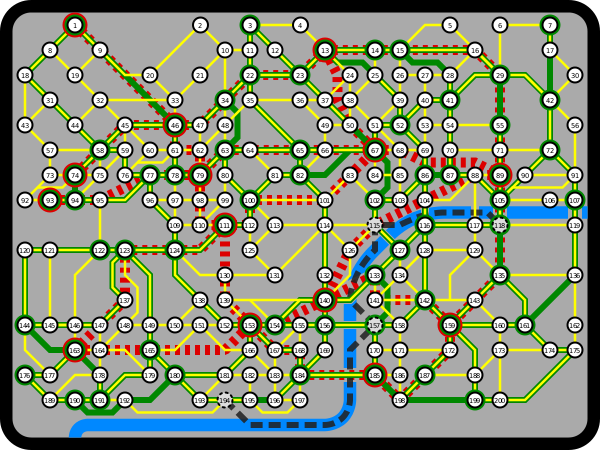
\includegraphics[width=0.9\textwidth]{obrazky-figures/scotland_original}
	\caption{Ukázka herní mapy hry Scotland Yard.
  Zdroj:\cite{scotland_original_image}}\label{fig:figure}
\end{figure}

Každému hráči je na začátku hry přidělen pouze určitý počet jízdenek na tyto dopravní prostředky.
K využití dopravy je potřebná právě tato jízdenka.
Pokud ji hráč nemá, nemůže již tento způsob přepravy použít.
Hra se dělí na kola, ve kterých se hráči střídají.

Hlavní myšlenkou hry je, že po většinu kol je pozice Pana X je policistům utajena.
Odhaluje se jim pouze určená kola.
To znamená, že policisté musí odhadovat další kroky Pana X aby ho mohli polapit.
Tímto se ze hry Scotland Yard stává hra s nedokonalou informací, jelikož policisté nevidí přesnou pozici Pana X\@.
Tento fakt ji činí vhodnou pro studování a rozvíjení oboru umělé inteligence.



\section{Další hry s nedokonalou informací}\label{sec:dalsi-hry-s-nedokonalou-informaci}
V oblasti umělé inteligence hraje důležitou roli modelování a řešení her.
Hry představují abstraktní formalizaci konfliktních interakcí mezi aktéry, tzv.~hráči.
Klasická teorie her se zaměřuje na hry s úplnou informací, kde mají všechny strany v daném okamžiku přístup ke všem relevantním informacím z herního prostředí.
V praxi se však častěji setkáváme se situacemi kde jednotlivým stranám chybí určité informace.


\subsection{Bayesovské hry}
{\color {red} [PŘEPSAT]}\label{subsec:bayesovske-hry}


Tyto případy lze modelovat pomocí her s neúplnou informací, kde hráči nemají úplné znalosti o prostředí či soupeřích.
Neúplnou informaci můžeme sledovat například v:
\begin{itemize}
  \item \emph{Ekonomii} - kde se jedná o nedokonalou informaci o trhu, cenách, situačních výkyvech, atd.
  \item \emph{Armáda} - kde se jedná o neúplnou informaci o pozici nepřítele, jeho vybavení, strategii, cíli, atd.
  \item \emph{Sportovní hry} - kde se jedná o nedokonalou informaci o taktice soupeře, jeho schopnostech, atd.
\end{itemize}

\begin{definition}[Bayesovská hra]
\cite{Y_Narahari} je definována pěticí $(N, A_i, \theta_i, p(\theta_i), u_i)$, kde:

\begin{itemize}
\item $N$ je konečná množina hráčů, $N = \{1, 2, \ldots, n\}$.
\item $A_i$ je neprázdná množina strategií hráče $i$.
\item $\theta_i$ je neprázdná množina typů hráče $i$.
\item $p(\theta_i)$ je apriorní pravděpodobnostní rozdělení typu hráče $i$ na $\theta_i$.
\item $u_i: A_1 \times \cdots \times A_n \times \theta_1 \times \cdots \times \theta_n \rightarrow \mathbb{R}$ je výplatní funkce hráče $i$.
\end{itemize}
\end{definition}
Bayesovské hry představují formální rámec sloužící k modelování her s nedokonalou informací.

\subsection{Stratego}\label{subsec:stratego}

Stratego je desková strategická hra pro dva hráče, která se odehrává na hracím plánu rozděleném do políček a využívá se k ní sada figurek reprezentujících armádu.
Vychází z dřívějších her, jako je Šachy a Go, a kombinuje strategické plánování, taktické manévry.

Cílem hry je porazit soupeře nalezením a obsazením jeho vlajky.
Hráči to dělají tak, že se navzájem utkávají se svými figurkami na herním plánu.

Každý hráč má 40 figur, rozdělených do 11 hodností (generál, plukovník, skaut, atd.).
Hráči mají k dispozici také bomby, které mohou zničit jakoukoliv figuru, avšak nemohou se hýbat.
Minu může zničitt pouze horník.
Figury lze rozeznat jen z jedné strany, proto oponent neví o jakou figuru se jedná.


Hra začíná tím, že každý hráč rozmístí své figury na herní pole.
Hráči se střídají v tazích, kdy se snaží najít oponentovu vlajku.
Pokud hráč táhne na pole, kde se nachází oponentova figura, nastává souboj.
Souboj spočívá v odkrytí obou figur a vyhrává ta s vyšší hodností.
Figura, která vyhrála zůstává, poražená figura je odstraněna z hry.
Ve hře Stratego je důležité blafování a odhadování soupeřových tahů.

\begin{figure}[!h]
	\centering
	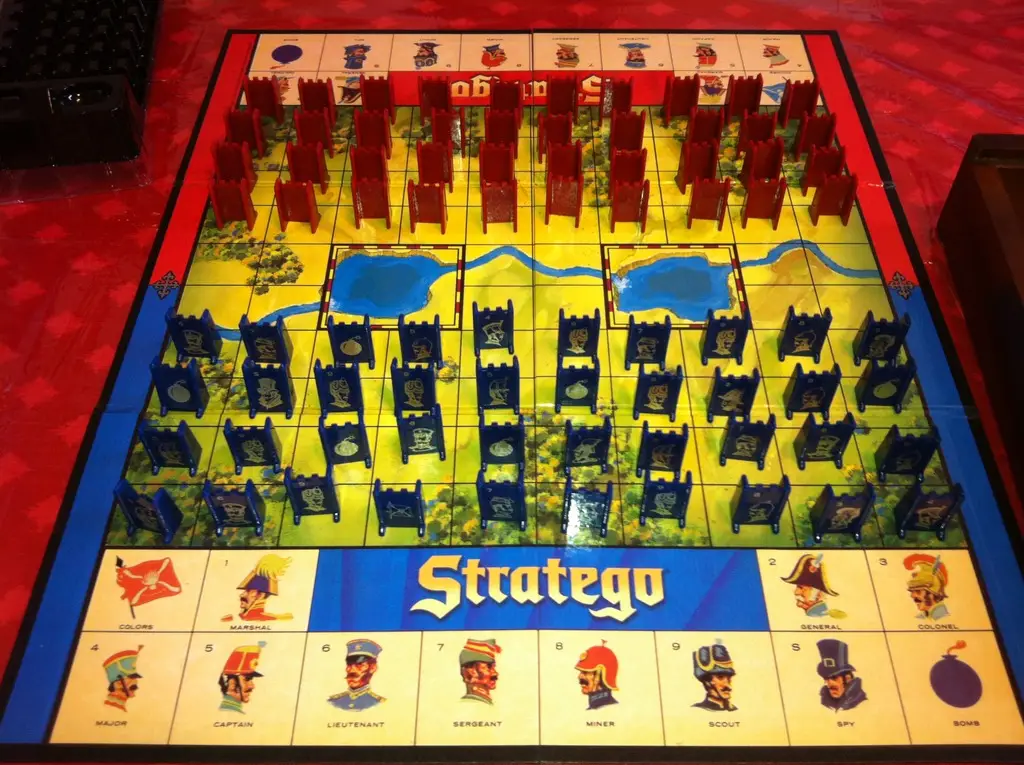
\includegraphics[width=0.6\textwidth]{obrazky-figures/stratego}
	\caption{Ukázka rozestavěných figur ve hře Stratego.
  Zdroj:\cite{Stratego_image}}\label{fig:figure2}
\end{figure}

Z pohledu umělé inteligence je Stratego zapeklitý problém.
Nejenže je hra s nedokonalou informací a je tedy zapotřebí odhadovat oponentovy tahy a blafovat.
Hra ale také má obrovský stavový prostor $10^{535}$\cite{Perolat_2022}.
Až do roku 2022 nebyla umělá inteligence v tétp hře moc úspěšná nedokázala se rovnat expertnímu hráče.
To se změnilo příchodem \emph{DeepNash}\cite{Perolat_2022}, kdy se tato metoda umístila mezi třemi nejlepšími hráči světa.

\subsection{Poker}\label{subsec:poker}


\section{Klíčové koncepty posilovaného učení}\label{sec:klicove-koncepty-posilovaneho-uceni}
Posilované učení (Reinforcement Learning, RL) je oblast strojového učení, která se zaměřuje na učení agentů v dynamickém prostředí.
Agent se učí strategii chování, která maximalizuje kumulativní odměnu.

\subsection{Agent}\label{subsec:agent}

Je komplexní entita, která interaguje s prostředím.
Prostředí poskytuje agentovi informace o stavu a agent na základě těchto pozorování vykonává akce.
Tyto akce mohou ovlivnit stav prostředí a agent obdrží odměnu na základě odměnové funkce.
Agent volí takové akce aby maximalizoval kumulativní odměnu.

\subsection{Prostředí}\label{subsec:prostredi2}

Je vše s čím agent interaguje.
Prostředí je buď fyzické (entity z reálného světa, ovládání chytré domácnosti, ovládání reaktoru, atd.) nebo virtuální (simulace, například hra).
Prostředí reaguje na akce agenta poskytuje mu zpětnou vazbu ve formě odměny či trestu (záporná odměna).
Pokud v prostředí existuje více agentů, může mít každý agent jiné pozorování.
Diky tomuto můžeme například schovat agentu \textit{A} určité informace, které agent \textit{B} vidí.

\subsection{Model}\label{subsec:model}

Je matematická funkce, která popisuje chování prostředí v závislosti na agentových akcích.
Model může být známý nebo neznámý, to následně rozděluje metody učení posilovaného na 2 základní kategorie: metody \emph{s modelem} a metody \emph{ bez modelu}.


\subsection{Politika}\label{subsec:politika}

Pomocí posilovaného učení vzniká takzvaná politika.
Politika je matematická funkce, která definuje agentovo chování na základě jeho pozorování (stavu).
Snaží se definovat takové chování, které vede k maximální kumulativní odměně.
Politika může být deterministická nebo stochastická.


  \subsubsection*{Deterministická politika}
  
  Deterministická politika přesně definuje cílový stav přechodu pro každý stav.
  Agent tedy pro jeden stav vždy volí stejnou akci.
  Tato politika je vhodná pokud je zapotřebí v každém stavu reagovat konzistentně, bez odchylek.
  Například, pokud agent ovládá termostat v domě a teplota je pod požadovanou hladinu.
  Nemůže se stát aby byla šance, že agent zvolí akci, která teplotu ještě sníží.
  Další výhoda, je že je jednoduchá na interpretaci a implementaci.\cite{Policies}

  Rovnice deterministické politiky je:
  \begin{equation}
    \pi(s) = a\label{eq:policy_deterministic}
  \end{equation}

  \subsubsection*{Stochastická politika}
  
  Zato stochastická politika definuje pro každý stav pravděpodobnostní rozdělení nad množinou akcí.
  Výsledná akce je tedy náhodná dle rozdělení pravděpodobnosti.
  Může tedy nastat situace kdy ve stejném stavu agent zvolí vždy jinou akci.
  Tato politika je vhodná v situacích, kdy je potřeba zkoumat různé strategie a kdy agent nemá úplnou informaci o prostředí.
  Například tam kde by deterministická politika zvolila jasnou akci \textit{A}, stochastická politika by mohla  s malou pravděpodobností zvolit akci \textit{B}.
  Čímž ale může odhalit, že stav \textit{B} je s ohledem na komulativní odměnu lepší než stav \textit{A}.\cite{Policies}

  Rovnice stochastické politiky je:
  \begin{equation}
    \pi(a \vert s) = \mathbb{P}_\pi [A=a \vert S=s]\label{eq:policy_stochastic}
  \end{equation}

  \subsection{Akce}\label{subsec:akce}

Akce je přechod z aktuálního stavu, do následujícího stavu z množiny možných stavů.
  Zjednodušeně, je to rozhodnutí, které agent vykonává v prostředí a toto rozhodnutí ovlivňuje prostředí.
  Akce zvolena dle politiky a je závislá na pozorování agenta.
  
  \subsection{Odměna}\label{subsec:odmena}

Odměna je hodnota, kterou agent obdrží od prostředí po vykonání akce.
  Může být kladná, záporná nebo nulová.
  Dle této zpětné vazby se agent učí, jak moc byla jeho zvolená akce v daném stavu vhodná.

\subsection{Hodnotová funkce}\label{subsec:hodnotova-funkce}

Hodnotová funkce vyhodnocuje, jak dobrý je stav tím, že predikuje budoucí odměnu.
  Čím vzdálenější odměna je, tím více je snížena.
  Jelikož, čím je odměna vzdálenější tím více je nejistá.

  Existují dva typy hodnotových funkcí:

  \subsubsection*{Hodnotová funkce stavu $V(s)$}

  Hodnotová funkce stavu \emph{$V(s)$} vyhodnocuje očekávanou komulativní odměnu, pokud se agent nachází v tomto stavu.
  Tato funkce je závislá na politice, kterou se agent řídí.
  Vyhodnocuje tedy jak příznivý je daný stav pro agenta.

  \subsubsection*{Hodnotová funkce akce $Q(s, a)$}
  \label{subsubsec:q_function}

  Hodnotová funkce akce \emph{$Q(s, a)$} vyhodnocuje očekávanou komulativní odměnu, pokud se agent nachází v tomto stavu a zvolí tuto akci.
  Tato funkce je opět závislá na politice, kterou se agent řídí.
  Vyhodnocuije tedy jak příznié je zvolení dané akce v aktuálním stavu.


\subsection{Markovský rozhodovací proces}\label{subsec:markovsky-rozhodovaci-proces}

Teměř všechny problémy, řešené posilovaným učením, mohou být označeny jako Markovy rozhodovací procesy (Markov Decision Process).
Tato abstrakce je základním kamenem pro modelování algoritmů posilovaného učení.
Markovský rozhodovací proces značí, že následující stav není závislý na stavech minulých, nýbrž pouze na aktuálním stavu.

\begin{figure}[!h]
	\centering
	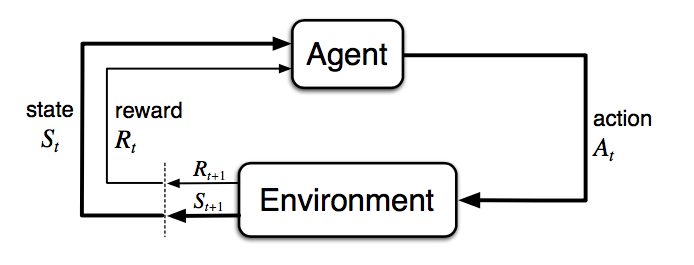
\includegraphics[width=0.6\textwidth]{obrazky-figures/RL_basics}
	\caption{Interakce mezi prostředím a agentem podle Markova rozhodovacího procesu.
  Zdroj:\cite{RL_basics}}\label{fig:markov}
\end{figure}

\begin{definition}
  
Markovský rozhodovací proces je definován pěticí $(S, A, P, R, \gamma)$\cite{RL_basics}, kde:

\begin{itemize}
\item $S$ je množina stavů.

\item $A$ je množina akcí.
\item $P$ je pravděpodobnostní přechodová funkce
\item $R$ je odměnová funkce
\item $\gamma$ je diskontní faktor pro budoucí odměny
\end{itemize}
\end{definition}

\subsection{Bellmanova rovnice}\label{subsec:bellmanova-rovnice}

Belmanova rovnice se zamuřuje na rozložení hodnotových funkcí na menží snadněji zpracovatelné celky.
Dociluje toho tak, že rozděluje hodnotovou funkci na dvě části: \emph{okamžitou odměnu} a postupně snižovanou \emph{budoucí odměnu}.

\begin{equation}
  V(s) = E[R_{t+1} + \gamma V(S_{t+1}) | S_t = s]\label{eq:bellman1}
\end{equation}

\begin{equation}
  Q(s, a) = E[R_{t+1} + \gamma E_{a\sim\pi}Q(S_{t+1}, a) | S_t = s, A_t = a]\label{eq:bellman2}
\end{equation}

\subsection{Rovnováha mezi explorací a exploatací (exploration-exploitation dillemma)}
\label{subsec:exploration-exploitation-dillemma}~\cite[Kompromis mezi potřebou získávat nové znalosti a potřebou použít již nabyté znalosti k vylepšení výkonnosti je jedním z nejzákladnějších kompromisů v přírodě]{Exploitation_Exploration}.
Explorace a exploatace jsou dvě protichůdné strategie, které se vyskytují jak ve strojovém učení tak i v reálném životě.

\emph{Exploatace} se snaží vybrat nejlepší možnou akci na bázi známých informací.
Tyto informace, nemusí být kompletní, nebo mohou být zavádějící.
A to z důvodu nedostatečného trénování, či nedostatečného prozkoumávání možností prostředí.

Tomu opačná metoda \emph{explorace} se snaží prozkoumat možnosti, které nejsou známé a mohly by vést k lepší budoucí odměně.

\subsection{Druhy informací v teorii her}\label{subsec:druhy-informaci-v-teorii-her}
V rámci umělé inteligence se potýkáme s různými druhy informací.
Dělí se na tyto hlavní typy:

\textbf{\emph{Dokonalá informace}} znamená, že agent ví o prostředí a o ostatních hračích vše.
Například ve hře šachny.
Hrač vidí všechny figury na herní ploše, i ty soupeřovy.

\textbf{\emph{Kompletní informace}} značí, že agent je obeznámen se strukturou hry a jsou mu také odhaleny odměnové funkce ostatních hráčů.
Hráč tedy ví jakou hru hraje je obeznámen s jejímy pravidly.
A rozumí jaké jsou podmínky výhry a je obeznámn s taktikou ostatních hráčů.

\textbf{\emph{Nedokonalá informace}} znamená, že agent nemá všechny relevantní informace o prostředí a ostatních hráčích.
Například, tedy všechny hry ve kterých hrají hráči zároveň jsou hry s nedokonalou informací.
Jelikož hráč v daném okamžiku nezná informaci o tahu ostatních hráčů.
Další příklad je například hra poker, kde hráč nezná rozdané karty ostatních hráčů.
Také hra Scotland Yard, kde policisté neznají pozici Pana X\@.

\textbf{\emph{Neúplná informace}} znamená, že hráč nezná strukturu odměn, podstatu hry nebo její pravidla.
Hráč tedy nezná výchozí informace o hře.
Všechny hry s neúplnou informací se dají považovat za hry s nedokonalou informací.

\emph{Soukromá informace} je informace, která není dostupná ostatním hráčům.

\emph{Společná informace} je informace, která je dostupná všem hráčům.

Příklady
\begin{itemize}
  \item Nedokonalá ale kompletní informace - poker
    Karty ostatních hráču jsou skryté
    {\color {red} [DODĚLAT PŘÍKLADY]}


\end{itemize}


\section{Vhodné algoritmy k řešení her s nedokonalou informací}\label{sec:vhodne-algoritmy-k-reseni-her-s-nedokonalou-informaci}

Tato kapitola se zaměřuje na algoritmy, které jsou vhodné pro řešení her s nedokonalou informací, s důrazem na metody posilovaného učení a srovnáním s klasickými metodami jako Monte Carlo.

\subsection{Monte Carlo tree search}\label{subsec:monte-carlo-tree-search}
Metoda Monte Carlo tree search (MCTS) je heruistický algoritmus prohledávání.
Kombinuje stromové vyhledávání s principy posilovaného učení.
Je často využíván, je--li stavový prostor řešeného problém příliš velký a složitý na to, aby byl prohledán kompletně jinýmy metodamy, jako například minimax, či alfa-beta prořezávání.
Tyto \uv{tradiční} algoritmy nelze na mnoho problémů použít, jelikož by byly příliš pomalé a náročné na výpočet.

Tato metoda se také potýká s rovnováhou mezi explorací a exploatací (viz.~ sekce~\nameref{subsec:exploration-exploitation-dillemma}).
Explorací se strom rozrůstá do šířky, zatímco exploatací se strom prohlubuje.

MCTS se skládá z několika fází:
\begin{itemize}
  \item \emph{Selekce}

  Na základě aktuálního stavu se vybere další stav k prozkoumání.
  Pro tento výběr se využívají dvě strategie:
  
  \emph{Strom s horní mezí spolehlivosti} (Upper confidence bounds applied to trees, UCT) kombinuje průměrnou hodnotu uzlu a odměnu za exploraci.

  \label{epsilon_greedy}
  \emph{Chamtivá strategie $\epsilon$ } ($\epsilon--greedy strategy$) vybíra s pravděpodobností $\epsilon$ náhodný uzel, jinak volí uzel s nejvyšší hodnotou.
  Tato strategie se používá méně čašto než UCT\@.

  Obě tyto strategie se snaží o rovnováhu mezi explorací a exploatací.
  \item \textbf{\emph{Expanze}}

  V tomto kroku se vyhledávací strom rozšíří o nový uzel, který je výstupem z předchozího kroku.

  \item \textbf{\emph{Simulace}}

  Po této fázi je provedena náhodná simulace od nového uzlu až do konečného stavu.

  \item \textbf{\emph{Aktualizace}}
  
  Díky nově nabitým informacím ze simulace, se zpětnou propagací aktualizují hodnoty uzlů ve stromě.

\end{itemize}

\begin{figure}[!h]
	\centering
	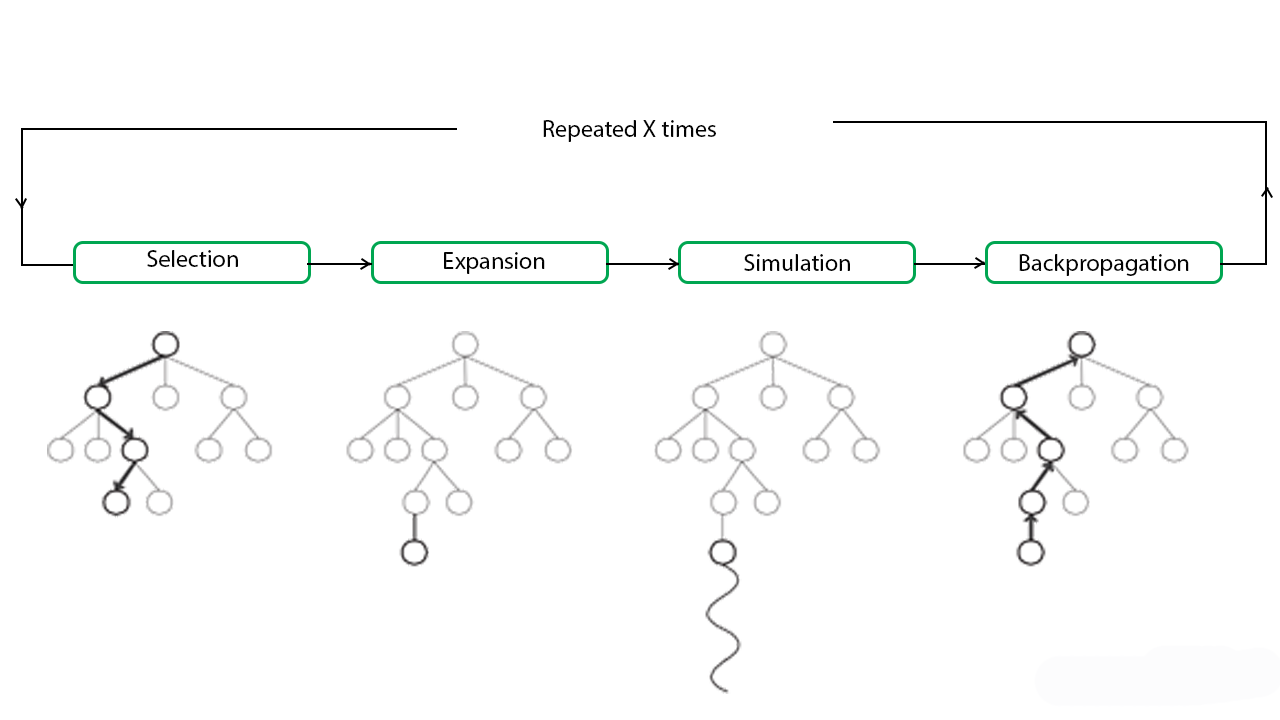
\includegraphics[width=0.9\textwidth]{obrazky-figures/mcts}
	\caption{Diagram jednotlivých fází MCTS.
  Zdroj:\cite{Monte_Carlo_Tree_Search}}\label{fig:mcts}
\end{figure}

Tento algoritmus se skvěle hodí na hry s nedokonalou či neúplnou informací, jelikož se spoléhá na vzorkování pomocí simulací.

\subsection{Q-learning}\label{subsec:q-learning}

Q-learning je jedním z nejznámějších algoritmů posilovaného učení.
Učení tohoto algoritmu probíhá bez modelu a mimo politiku.

Jak už název vypovídá, Q-learning se zaměřuje na určení hodnoty hodnotové funkci akce $Q(s, a)$, viz. \nameref{subsubsec:q_function}.
Pokud dostane kladnou odměnu po vykonání akce $s$, zvýší se hodnota $Q(s, a)$.
Naopak, dostane--li po vykonání této akce zápornou odměnu, hodnota $Q(s, a)$ se sníží.
Hlavním prvkem tohoto algoritmu je Q--tabulka, která na každou kompbinaci stavu a akce uchovává hodnotu $Q(s, a)$.
Řádky jsou tedy stavy a sloupce akce.
Na začátku jsou všechny $Q$ hodnoty v tabulce inicializovány na nulu.
Následně jsou tyto hodnoty iterativně aktualizovány dle zpětné vazby udělené od prostředí ve formě odměny.

Jako u většiny algoritmů je zde potřeba dohlédnout na rovnováhu mezi explorací a exploatací.
K tomuto se využívá $\epsilon$--greedy strategie viz. \nameref*{epsilon_greedy}.

Protože tato metoda mapuje $Q$ hodnoty pro každou kombinaci stavu a akce nastává zde problém.
Je--li stavový, či akční prostor příliš velký, nebo dokonce nekonečný je tento algoritmus nevhodný, skoro až nepoužitelný.
Jako řešení byl navrhnut algoritmus Deep Q-learning.

\subsection{Deep Q-learninggg}\label{subsec:deep-q-learninggg}

Tato metoda je rozšířením algoritmu Q-learning.
Místo mapovací $Q$--tabulky využívá hluboké neuronové sítě k aproximaci hodnotové funkce akce $Q(s, a)$.
Díky této aproximaci je možné použít tento algoritmus na problémy s velkým, či nekonečným stavovým prostorem.

Avšak tímto vzniká nový problém, \emph{nestabilita učení}.
Ten je řešen dvěma mechanizmy:

\begin{itemize}
  \item \textbf{\emph{Přehrání zkušenosti (experience replay)}}
  

  \item \emph{Periodická aktualizace}

  Síť je naklonována a změny se provádí pouze na duplikátní verzi.
  Do hlavní originální sítě se změny klonují po určitém počtu kroků.


\end{itemize}

\subsection{Gradient politiky}\label{subsec:gradient-politiky}
Oproti předchozím zmiňovaným algoritmům, které se snaží naučit hodnotovou funkci či prohledávají stavový prostor, algoritmy gradientu politiky se snaží naučit politiku přímo.

V diskrétním prostoru je odměnová funkce definována jako:
\begin{equation}
  \label{eq:odmenova_funkce}
  \mathcal{J}(\theta) = V_{\pi_\theta}(S_1) = \mathbb{E}_{\pi_\theta}[V_1]
\end{equation}

V spojitém prostoru je odměnová funkce definována jako:
\begin{equation}
    \label{eq:odmenova_funkce_spojita}
  \mathcal{J}(\theta) = \sum_{s \in \mathcal{S}} d_{\pi_\theta}(s) V_{\pi_\theta}(s) = \sum_{s \in \mathcal{S}} \Big( d_{\pi_\theta}(s) \sum_{a \in \mathcal{A}} \pi(a \vert s, \theta) Q_\pi(s, a) \Big)
  \end{equation}

\subsubsection*{Věta o gradientu politiky}
Výpočet gradientu matematicky je zaznamenán touto rovnicí:

\begin{equation}
  \label{eq:gradient_politiky}
  \frac{\partial \mathcal{J}(\theta)}{\partial \theta_k} \approx \frac{\mathcal{J}(\theta + \epsilon u_k) - \mathcal{J}(\theta)}{\epsilon}
\end{equation}
Tento výpočet je velmi pomalý a náročný na výpočet.
Avšak tento vzorec lze zjednodušit na rovnici zvanou \emph{věta o gradientu politiky}:

\begin{equation}
    \label{eq:veta_o_gradientu_politiky}
  \nabla \mathcal{J}(\theta) = \mathbb{E}_{\pi_\theta} [\nabla \ln \pi(a \vert s, \theta) Q_\pi(s, a)]
\end{equation}


\section{Zkoumaný algoritmus proximální optimalizace politiky}
\label{sec:proximalni-optimalizace-politiky}


\chapter{Zhodnocení současného stavu a plán práce (návrh)}
\label{ch:navrh}
\begin{itemize}
  \item \emph {Kritické zhodnocení dosavadního stavu}
  \item \emph {Návrh, co by bylo vhodné vyřešit na základě znalostí dosavadního stavu}
  \item \emph {Co jste konkrétně udělal s teorií popsanou výše}
  \item \emph {Volba OS, jazyk, knihovny}
  \item \emph {Detailní rozbor zadání práce, detailní specifikace a formulace cíle a jeho částí}
  \item \emph {Popis použití řešení, situace/problémy, které projekt řeší}
  \item \emph {Postup práce/kroky vedoucí k cíli, rozdělení celku na podčásti}
  \item \emph {Návrh celého řešení i jeho částí, s odkazy na teoretickou část}
\end{itemize}

\section*{Zkoumaná modifikovaná verze hry Scotland Yard}

Tato práce využívá modifikovanou verzi hry Scotland Yard, ve které se hráči pohybují po mřížkové herní ploše ve tvaru čtverce.
Na mřížce se nachází {\color{red}[15x15]} polí.
Hračí se po těchto polích pohybují ortogonálně i diagonálně, vždy o maximálně 1 pole.
Hráč se může rozhodnot nezměnit pozici a zůstat na svém aktuálním poli.
K pohybu nejsou potřebné žádné jízdenky.
Toto zjednodušení herní plochy nijak nemění základní podstatu hry, zachovává neurčitost, ale značně zjednodušuje implementaci.

Předtím nežli začne hra, že se vyberou náhodné možné pozice Pana X a policistů.
Z těchto možných pozíc se následně náhodná pozice přidělí jednotlivým hráčům.
Poté začíná hra.
Hra se dělí na jednotlivá kola, ve kterých se hráči střídají.
Pro hru byli zvoleni 3 policisté z toho důvodu, že je herní pole velmi velké a 2 policisté by nemuseli mít možnost ho celé pokrýt.
V kole hraje jako první Pan X a poté policisté, již podle jejich očíslení, které jim bylo přiděleno při vytváření.
Hra končí v okamžiku, kdy policisté chytí Pana X nebo když Pan X zůstane nepolapen až do konce.

\section*{Implementace umělé inteligence do hry Scotland Yard pomocí algoritmu PPO}
\label{sec:implementace}

\subsection{Použité technologie}\label{subsec:pouzite-technologie}
K učení politiky pro hru Scotland Yard byla využit open-source framework \emph{Ray}~\cite{Ray}.
Konkrétně byla využita knihovna \emph{Ray.Rllib}.
Tato knihovna poskytuje nástroje pro posilované učení a samotné implementace jednotlivých algoritmů, včetně zkoupameného algoritmu \emph{PPO}.
Rllib dokáže využívat obě populární knihovny pro strojové učení \emph{Tensorflow} a \emph{Pytorch}.
Pro tuto práci byla vybrána knihovna \emph{Pytorch}.

Před finálním rozhodnutím pro využití frameworku Ray byly zkoumány i další možnosti.
{\color{red}[Dopsat]}
Knihovna Stable Baselines 3.
Knihovna byla zavrhnuta, jelikož neumožňuje učení více politik se hraním agentů proti sobě.

\subsection{Implementace uživatelského rozraní a herních mechanizmů}\label{subsec:implementace-uzivatelskeho-rozrani-a-hernich-mechanizmu}

Uživatelské rozhraní bylo vytvářeno pomocí knihovny \emph{Pygame}.
Hra začíná v menu, kde je momentálně možné vybrat pouze možnost sledování hry mezi dvoumy agenty.
Je zde ale možnost vybrat jaký algoritmus rozhodování je použit, jestli algoritmus PPO či náhodné chování.

Samotný kód hry je rozdělena na 3 částí.

\begin{itemize}
  \item \emph{GameController}~\cite{GameSceneController}
  
  Tato třída je zodpovědná za řízení hry.
  Je zde spuštěna univerzální herní smyčka která zpracovává uživatelské vstupy.
  A následně provádí aktualizaci stavu aktuální scény a překreslení dané scény.
  \item \emph{Scény}~\cite{GameSceneController}
  
  Jednotlivé scény následně definují své chování při aktualizaci a překreslení.
  Manipulace a přepínání mezi nimy je zajištěno pomocí zásobníků scén.
  Do tohoto zásobníku se ukládájí nově otevřené scény a obsluhována je vždy ta nejnovější.

  \item \emph{Hra}
    Samotná hra je následovně rozdělena na 2 podčástí která každá zpracovává jinou stránku hry.
    \begin{itemize}
      \item \emph{Herní logika} src/game/scotland\_yard\_game\_logic.py
      Zpracovává herní mechanizmy, jako je pohyb, zpracování výherních podmínek, atd.
      Zprostředkovává informace pro prostředí a to poté pro učící se agenty.

      \item \emph{Herní vizualizace}  src/game/scotland\_yard\_game\_visual.py
      Vykreslování herních elementů (herní pole, figury, atd.).
    \end{itemize}
\end{itemize}

\textit{Použití herní smyčky, která obsluhuje aktuální scénu byl inspirován tutoriálovým projektem z platformy GitHub \cite{GameSceneController}.
Kód byl avšak značne upraven a vylepšen aby vyhovoval integrování do této práce.}

Jednotlivé vrstvy hry jsou tak izolovány a mohou být snadno vyměněny za jiné implementace.

\subsection{Prostředí}\label{subsec:prostredi}
Vytvořit prostředí pro platformu Ray.Rlib byl velký oříšek.
Dokumentace vytváření prostředí není příliš komplexní, byl tedy problém zajistit správnou komunikaci prostředí a agentů.
Prostředí je komplikovanější, jelikož zde figuruje více agentů a dvě rozdílne strategie (politiky).

\subsubsection*{Řešení zvolení nevalidních akcí}

Hra Scotland Yard má omezené herní pole.
Tím pádem je jasné, že pokud jsou hráči na okraji herního pole, nemohou zvolit takovou akci, která by je posunula mimo herní pole.
K vyřešení tohoto problému se využívá tzv.~ maska akcí (\emph{Action mask}).
Framework Ray tuto možnost v omezené míře podporuje.
Je avšak potřeba vytvořené prostředí obalit v obalové třídě, která tuto funkcionalitu zprostředkuje.
Avšak nepodařilo se mi tuto funkcionalitu zkloubit s dalšímy požadavky systému.
Mezi těmito požadavky je fungování více aktérů s různými politikami v jednom prostředí a různé pozorovací prostory agentů.

Politika, tedy může zvolit nevalidní akci, ale je velmi penalizována.
Agenti ji tedy zvolí opravdu zřídka.
Pokud se tak stane, je ve hře implementovaná funkcionalita, která se pokusi znovy vygenerovat akci, dokud není validní.
Aby se zamezilo nekonečnému cyklu čekání na validní akci, je po 100 pokusech vygenerována náhodná validní akce.
Takto uměle generovaná akce, nebyla za celou dobu testování potřeba.

\subsubsection*{Systém odměn}

Jednotlivým agentům jsou udělovány odměny na základě jejich chování.
Jelikož policisté a Pan X mají odlišné protichůdné i jejich odměny jsou odlišné.

\begin{equation}
    \label{eq:odmena_za_vzdalenost_od_policistu}
  R_{\rho_p} = \sum_{i=1}^{3}[(\rho_{p_i} - \rho_{pref}) \div 3]
\end{equation}
\begin{equation}
    \label{eq:odmena_za_vzdalenost_od_posledni_pozice}
  R_{\rho_l} = \rho_l * 0.2
\end{equation}
  \begin{equation}
    \label{eq:celkova_odmena}
  R = R_{\rho_p} + R_{\rho_l}
\end{equation}

\begin{itemize}
  \item $R_{\rho_p}$ - odměna za vzdálenost od policistů
  \item $R_{\rho_l}$ - odměna za vzdálenost Pana X od jeho poslední známé pozice
  \item $R$ - celková odměna
  \item $\rho_l$ - vzdálenost Pana X od jeho poslední známé pozice
  \item $\rho_{p_i}$ - vzdálenost policisty $i$ od Pana X
  \item $\rho_{pref}$ - pomezí mezi kladnou a zápornou odměnnou.
  Pokud je vzádelenost od policisty menší než tato hodnota, Pan X obdrží záporno odměnu a naopak kladnou.
\end{itemize}

Výpočet odměny policistů je složitější.
Policisté znají poslední odhalenou pozici Pana X\@.
Okolo tohoto bodu je vytvořená oblast, ve které se Pan X může nacházet.
Policisté znají nejbližší bod této oblasti.
Pokud je policista v této oblasti dostáva odměnu.
Pokud je mimo tuto oblast zájmu, je penalizován.
Čím blíže je policista k této oblasti tím menší penalizaci obdrží.

Tento styl odměnování policistů se ukázal jako velmi efektivní.
Další varianta byla přidat do pozorování policistů pozice všech políček, kde se může Pan X nacházet.
Toto by ale bylo velmi neefektivní, jelikož by se pozorovací prostor několikanásobně zvětšil.
Tím by se zvýšila náročnost výpočtů a zpomalilo by se učení.

\subsubsection*{Pozorování agentů}

\chapter{Experimenty}
\label{ch:experimenty}
\chapter{Závěr}
\label{ch:zaver}
\chapter{Přílohy}
\label{ch:prilohy}



%===============================================================================

% Pro kompilaci po částech (viz projekt.tex) nutno odkomentovat
%\end{document}
